% ****** Start of file apssamp.tex ******
%
%   This file is part of the APS files in the REVTeX 4.1 distribution.
%   Version 4.1r of REVTeX, August 2010
%
%   Copyright (c) 2009, 2010 The American Physical Society.
%
%   See the REVTeX 4 README file for restrictions and more information.
%
% TeX'ing this file requires that you have AMS-LaTeX 2.0 installed
% as well as the rest of the prerequisites for REVTeX 4.1
%
% See the REVTeX 4 README file
% It also requires running BibTeX. The commands are as follows:
%
%  1)  latex apssamp.tex
%  2)  bibtex apssamp
%  3)  latex apssamp.tex
%  4)  latex apssamp.tex
%
\documentclass[%
 reprint,
%superscriptaddress,
%groupedaddress,
%unsortedaddress,
%runinaddress,
%frontmatterverbose,
%preprint,
%showpacs,preprintnumbers,
%nofootinbib,
%nobibnotes,
%bibnotes,
 amsmath,amssymb,
 aps,
%pra,
%prb,
%rmp,
%prstab,
%prstper,
%floatfix,
]{revtex4-1}

\usepackage[utf8]{inputenc}
\usepackage[norsk]{babel}
\usepackage{varioref}
\usepackage{graphicx}% Include figure files
\usepackage{dcolumn}% Align table columns on decimal point
\usepackage{bm}% bold math
\usepackage[margin=0.4in]{geometry}
\usepackage[mathlines]{lineno}% Enable numbering of text and display math
%\linenumbers\relax % Commence numbering lines

\usepackage[usenames,dvipsnames,svgnames,table]{xcolor}
\usepackage[colorlinks]{hyperref}
\usepackage{relsize}
\usepackage{amsmath,graphicx,verbatim,amsfonts,geometry}
\newcommand*\diff{\mathop{}\!\mathrm{d}}
\newcommand*\Diff[1]{\mathop{}\!\mathrm{d^#1}}
\usepackage{ulem}
\usepackage{amssymb}
\usepackage{soul}
\usepackage{dsfont}
\usepackage{commath}
\usepackage{wrapfig}
\usepackage[free-standing-units=true]{siunitx}
\DeclareSIUnit\year{yr}
\usepackage{gensymb}
\newcommand{\ROM}[1]{%
  \textup{\uppercase\expandafter{\romannumeral#1}}%
}
\usepackage{physics}
\usepackage{caption}
\usepackage{bm}

%\usepackage[showframe,%Uncomment any one of the following lines to test
%scale=0.7, marginratio={1:1, 2:3}, ignoreall,% default settings
%text={7in,10in},%centering,
%margin=0.1in,
%total={6.5in,8.75in}, top=1.2in, left=0.9in, includefoot,
%height=10in,a5paper,hmargin={3cm,0.8in},
%]{geometry}

\begin{document}

%\preprint{APS/123-QED}

\title{Måling av multimetere, temperaturmåling med termistor\\ og kretser med frekvensavhengig respons}

\author{\textsc{Haugerud, Ivar Svalheim}}
\affiliation{%
 University i Oslo\\
}%

\date{\today}

\begin{abstract}
Vi gjorde målinger på elektriske kretser og fant at den indre motstanden til F$45$ og F$75$ som voltmeter er henholdsvis $10.00\pm0.06$M$\Omega$ og $11.10\pm0.07$M$\Omega$. Dette må vi ta i betrakting når vi skal måle spenningsfallet over en motstand med resistanse av samme størrelsesorden som voltmeteret. Vi målte denne effekten og merket en kraftig forskjell på $0.08$M$\Omega$. For at F$45$ og F$75$ skal kunne måle motstand og strøm direkte må de selv sende de selv en strøm inn i kretsen. Av å sende en vekselstrøm i målte vi at den avleste verdien på et multimeter er lik RMS-verdien til signalet fra spenningsgeneratoren. En krets med vekselstrøm av høy frekvens og en kondensator, fungerer som et lavpass filter, siden signalene med høy frekvens vil bli redusert logaritimisk lineært med logaritmen av frekvensen. Eksperimentet viste at den karakteristiske frekvensen til systemet var $118.54 \pm  0.68$Hz. Dette stemmer ikke overens med hva teorien forutsier, og det burde derfor bli gjort flere eksperimenter på dette området.
\end{abstract}

\pacs{Valid PACS appear here}% PACS, the Physics and Astronomy
                             % Classification Scheme.
%\keywords{Suggested keywords}%Use showkeys class option if keyword
                              %display desired
\maketitle

%\tableofcontents
\section{\label{introduksjon}Introduksjon}
Eksperimentet diskutert i denne rapporten ble gjennomført i håp om å finne ut av, og forstå, samspillet mellom komponenter, og effekten komponentene og måleapparatene har på kretsen de er en del av. De følgende kretsene vi skal se på ble lagd for å teste denne effekten. Spenningen i kretsen vil være generte av DA-omformere og oscilloscop, dette lar oss variere frekvens og amplitude som vi ønsker. Dette vil bli målt av multimetere, AD-omformere og oscilloscop. Kretsen kommer i all hovedsak til å bestå av resistanser, kondensatorer og termistorer. Med disse komponentene og måleapparatene kan vi måle hvordan kompoentene oppfører seg i samspill for forskjellige amplituder og frekvenser. Spesielt vil vi se på hvordan kondensatorer oppfører seg for høye og lave frekvenser, og vi kan sammlikne målingene med hva teorien fra Ohm's lov, sammen med kirchhoffs lover, forutsier at resultatene skal være.
\section{\label{teori}Teori}
Vi jobber med elektriske kretser hvor vi bruker Ohm's lov \cite{skaar} for å regne på kretsene våre
\begin{equation}
  V = IR \label{ohm},
\end{equation}
hvor $V$ er spenningsfallet over en komponent, $I$ er strømmen som gjør gjennom komponenten, og $R$ er resistansen til komponenten. Dette gir oss forholdet mellom motstand, strøm og spenningsfall, som er nødvendig for en hver krets. Denne formelen kommer vi til å bruke mye gjennom forsøket siden vi kan finne resistansen ved å måle spenningsfallet over en komponent når vi vet hva strømmen er. Dette blir spesielt nyttig hvis resistansen til en komponent er avhengig av temperaturen i rommet. \\
I kretsene våre kommer vi til å bruke kondensatorer. Kondensatorer kan lagre elektriske ladninger med netto ladning $Q$, dette generer et spenningsforskjell mellom kondensatorplatene $V$. Disse to egenskapene til kondensatoren gir oss kapasitansen til kondensatoren som er gitt av
\begin{equation}
  C = \frac{Q}{V},
\end{equation}
hvor $C$ er kapsitansen. Kapasitansen er bare avhengig av materialet og de geometriske strørrelsene til kondensatorplatene \cite{skaar}. Kapasitansen sier oss hvor mye ladning kondensatoren klarer å oppbevare før den blir \textit{full}. Hvis man kobbler inn en resistanse i kretsen også, slik at man får en RC-krets, vil man ha lagd et lavpassfilter. Grunnen til dette er at forflyttingen av ladninger i kretsen tar tid, og gjør at, hvis man har en vekselstrøm (AC) vil spenningen over kondensatoren være en funksjon av tid, og med for stor frekvens på strømmen vil ikke strømmen i kretsen ha tid til å fylle opp kondensatoren med ladninger før strømmen endres igjen. Og derfor vil man ha en høy frekvens som går inn i kondensatoren, men en lav frekvens som går ut av kondensatoren. Forholdet mellom spenningen inn $V_i$ og spenningen ut $V_u$ kan vises at \cite{oppgave} er
\begin{equation}
  \abs{\frac{V_u}{V_i}} = \frac{1}{\sqrt{1+\left(\frac{\omega}{\omega_0}\right)^2}}
\end{equation}som, ved å ta logaritmen på begge sider, kan skrives om til
\begin{equation}
  \log\abs{\frac{V_u}{V_i}} = -\frac{1}{2}\log\left\{1+\left(\frac{\omega}{\omega_0}\right)^2 \right\}
\end{equation}
Her har spenningen inn en frekvens $\omega$ og $\omega = 1/RC$, som er den karakteristiske frekvens til kretsen. For lave frekvenser ser vi at $\log\abs{V_u/V_i}\approx 0$. For høye frekvenser ser vi at $\log\abs{V_u/V_i}\approx -\log(\omega) + log(\omega_0)$, som, hvis plottet med logaritmiske akser, er en rett linje med konstantledd $\log(\omega_0)$ og stigningstall $-1$, der $x$-aksen er $\omega$ og $y$-aksen er $\abs{V_u/V_i}$. Dette betyr at den relative amplituden faller en faktor $10$ for hver faktor $10$ vi øker frekvensen. Dette gjør at de høye frekvensene vil falle bort, som gjøre kretsen til et lavpassfilter.
\\
Når vi jobber med vekselstrøm (AC) er man ofte interesert i effektverdien, eller RMS-verdien til signalet. Denne verdien er definert som
\begin{equation}
  V_{rms} = \sqrt{\frac{1}{T} \int_0^T V(t)^2 \diff t} \label{rms},
\end{equation}hvor $T$ er tiden for en full periode og $V(t)$ er spenningen i kretsen. Hvis man løser dette integralet for forskjellige signalformer får man RMS-verdien. De signalen vi skal se på er sinussignal, firkantsignal og sagtann signal, det kan vises at RMS-verdiene til signalene er henholdsvis lik $A/\sqrt{2}$, $A$, $A/\sqrt{3}$, hvor $A$ er amplituden av signalet \cite{rms_wiki}.
\\
Et av eksperimentene går ut på å måle resistansen til en temperatursensitiv termistor, der motstanden er en funksjon av temperatur, og ut ifra målingene av resistansen måle temperaturen. Utrykket for dette forholdet er
\begin{equation}
  T(R) = \frac{1}{a+b\, \log R + c \left(\log R\right)^3} - 273.16 \degree\text{C} \label{calc_temp}
\end{equation}hvor $a$, $b$ og $c$ er konstanter. Her sender vi med en resistanse, og får ut en temperatur målt i celcius. \\
For å beregne hvordan usikkerhetene går videre i målingene brukte vi formlene \cite{squires} vist nedenfor
\begin{align*}
  Z = A \pm B &\rightarrow \left(\Delta Z\right)^2 =  \left(\Delta A\right)^2 +\left(\Delta B\right)^2 \\
  Z = A\cdot B &\rightarrow \left(\frac{\Delta Z}{Z}\right)^2 =  \left(\frac{\Delta A}{A}\right)^2 +\left(\frac{\Delta B}{B}\right)^2 \\
  Z = \frac{A}{B} &\rightarrow \left(\frac{\Delta Z}{Z}\right)^2 =  \left(\frac{\Delta A}{A}\right)^2 +\left(\frac{\Delta B}{B}\right)^2
\end{align*}
\section{\label{metode1}Metode}
\subsubsection*{Utstyrsliste}
\begin{itemize}
\item Breadboard
\item To motstandere $10\Omega$ og $1$M$\Omega$
\item Termistor
\item Fluke 75 Håndhold multimeter
\item Flue 45 Lab-multimeter
\item Variabel spenningskilde, $\pm 15$ V
\item Oscilloscop med innebygd funksjonsgenerator (PicoScope 2000 Series)
\item PC med AD/DA-omformer (NI USB-6211) og Matlab installert
\item Løse ledninger (enkeltledere) for å koble fra AD/DA-omformer til breadboard
\item Koaks-kabel med BNC i hver ende
\item To BNC-til-banan-overganger
\item En BNC-forgreining
\item $100$ nF kondensator og 10 k$\Omega$ motstand
\end{itemize}
\subsection{Måling av multimetere}
Vi ønsket å finne ut hvordan det å måle motstand, strøm eller spenning påvirker kretsen som måleapparatet er med i. For å gjøre dette brukte vi to multimetere Fluke $75$ (F$75$) som er et håndholdt multimeter, og Fluke $45$ (F$45$), som er et stasjonert multimeter. Vi lot multimeterene måle på hverandre i en ekstremt simpel krets der måleapparatene er de eneste komponentene i kretsen, dette er vist i figur \ref{fig1}. Dette gjorde vi for alle kombinasjonene av resistans, strøm og spenning i kretsen, og varierte sensitiviteten og samplings-frekvensen (slow (S), medium (M) og fast (F)) til måleapparatene. \\
\begin{figure}[h!]
    \centering
    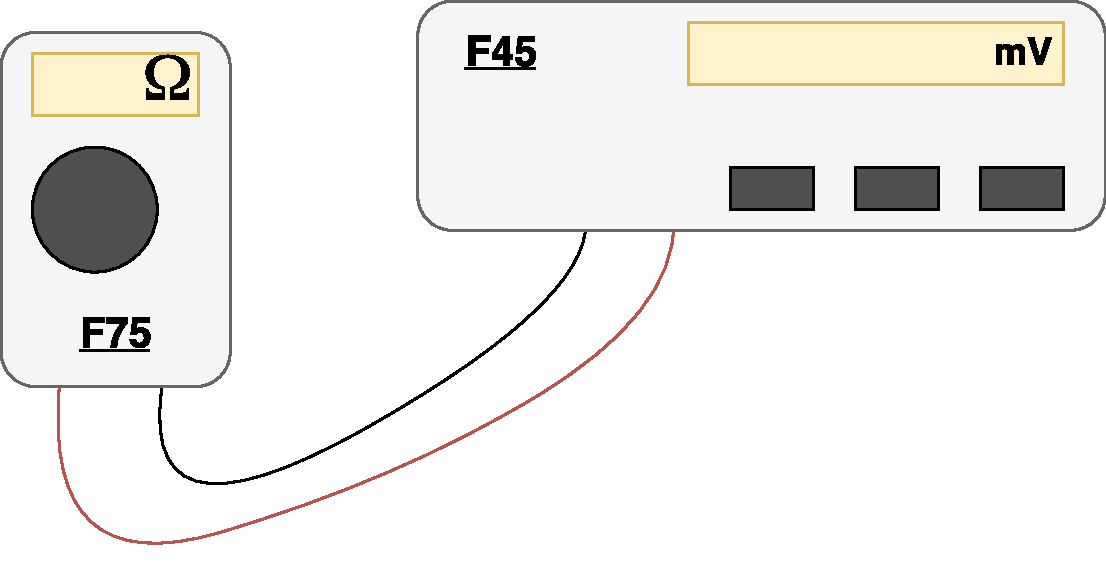
\includegraphics[scale=0.35]{fig_1.pdf}
    \caption{Figur som viser F$45$ og F$75$ som måler på hverandre i en veldig simpel krets. I dette eksempelet måler F$75$ resistansen gjennom kretsen, mens F$45$ måler spenningen.}
    \label{fig1}
\end{figure}
\subsection{Motstand, likestrøm og likespenningsmålinger med multimeter}
Nå som vi viste hvordan måleapparatene påvirket krets de selv er med i brukte vi dem til å måle resistansen til to motstander hvor vi vist den eksakte verdien av resitansen. Dette gjorde vi ved å sette opp en enkel krets vist i figur \ref{fig2} ved hjelp av et breadbord.
\begin{figure}[h!]
    \centering
    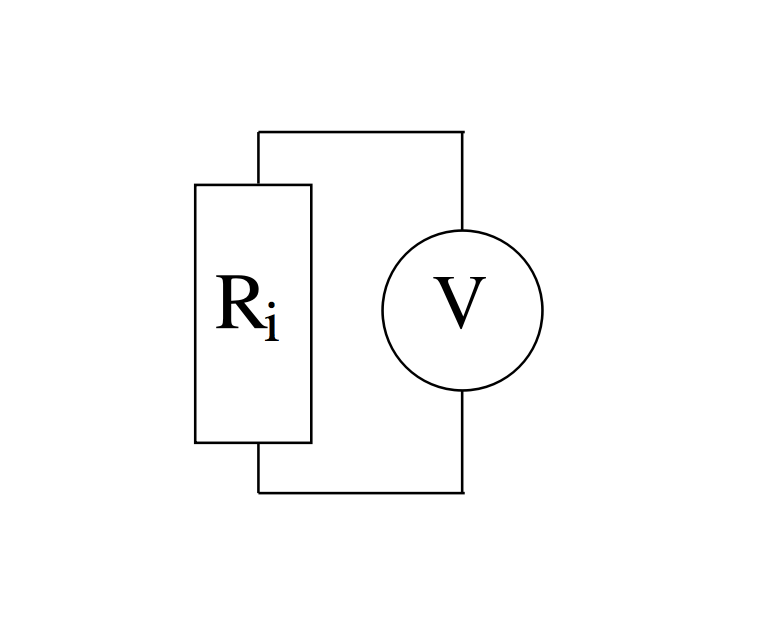
\includegraphics[scale=0.15]{fig_2.png}
    \caption{Krets brukt for å måle resistansen til motstander der vi kunne variere $R_i$.}
    \label{fig2}
\end{figure}
Vi valgte denne kretsen siden dette var den letteste mulige kretsen for hensikten vår. Vi brukte to forskjellige resistanser i kretsen, først $R_1 \sim 10 \Omega$ og så $R_2 \sim 1 M\Omega$. Vi gjorde først målingene med F$75$ og så med F$45$. Hvor begge appartene brukt ohm-funksjonen, slik at de genererte strømmen i kretsen selv.

\subsection{Automatiserte målinger av termistor-motstand}
Vi ønsket så å utvide kretsen og gjøre den litt mer komplisert. Kretsen vi lagde er vist i figur \ref{fig3}.
\begin{figure}[h!]
    \centering
    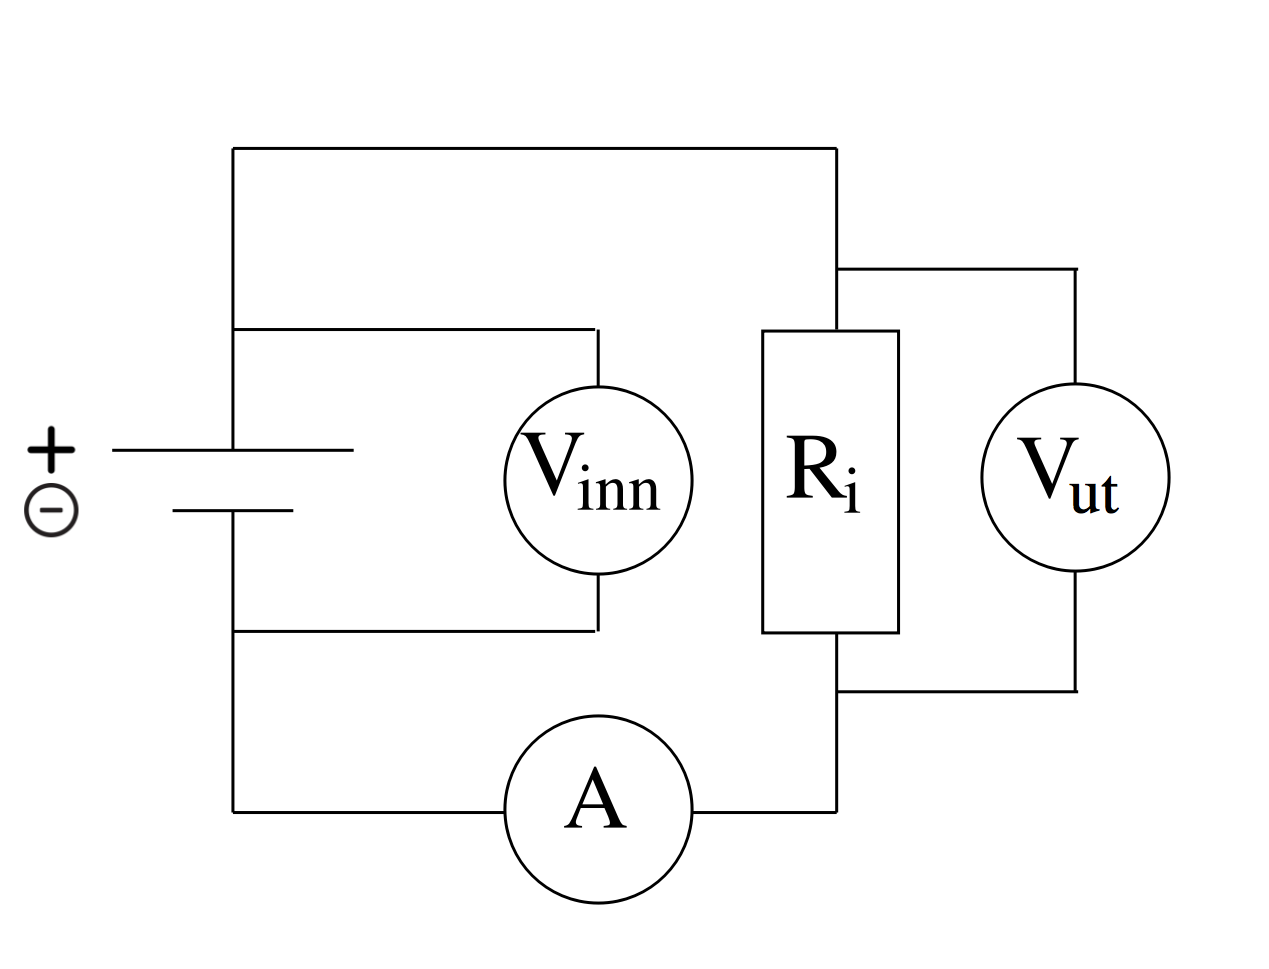
\includegraphics[scale=0.15]{fig_3.png}
    \caption{Krets brukt for å måle resistansen til motstander der vi kunne variere $R_i$.}
    \label{fig3}
\end{figure}
I denne kretsen måler vi spenningsfallet over hele kretsen ved $V_{inn}$, spenningsfallet over resistansen ved $V_{ut}$, og strømmen som går gjennom kretsen ved amperemeteret. Med disse målingene kan vi regne ut resistansen til motstanden. Siden vi hadde to mutlimetere, og tre verdier vi ønsket å måle i kretsen måtte vi koble om kretsen under forsøket for å gjøre de forskjellige målingene. Når alt var riktig koblet opp varierte vi strømmen i kretsen, og gjorde målinger for begge resistanser for hver frekvens. Da vi gjorde målinger med $R=\SI{10}{\ohm}$ brukte vi F$45$ som voltmeter, og F$75$ som amperemeter. Når vi gjorde de samme målingene for $R=\SI{1}{\mega \ohm}$ måtte F$45$ være amperemeter, siden F$45$ hadde høyere sensitivitet, og kunne derfor gi målinger på den lave strømmen i kretsen. I kretsen vår brukte vi F$45$ for å måle $V_{inn}$ og $V_{ut}$, mens vi brukte F$75$ som amperemeter, grunnen til dette var at det ga oss minst omkoblinger underveis.
\subsection{Vekselspenning med frekvensgenerator, oscilloscop og multimeter}
Vi ønsket nå å gjøre målinger ved hjelp av en datamaskin for å autmatisere målingene, og få en grafisk fremstilling av dataen. For å få dataen fra målingene inn på datamaskinen koblet vi tre fofrskjellige punkter i kretsen inn til en dataakvisisjonsboks (DAQ, NI USB-6211). I kretsen hadde vi en konstant spenning på $\SI{5}{\volt}$, og en termistor ($R_T$) og en resistans ($R_2$) koblet i serie. Mellom hver av resistansen koblet vi kretsen inn til akvisisjonsboks, kretsen er vist i figur \ref{fig4}. Her er $AIGND$, $AI0$, $AI1$ inngangene vi brukte på akvisasjonsboksen og referanse motstanden $R_2$ var på $1M\Omega$.
\begin{figure}[h!]
    \centering
    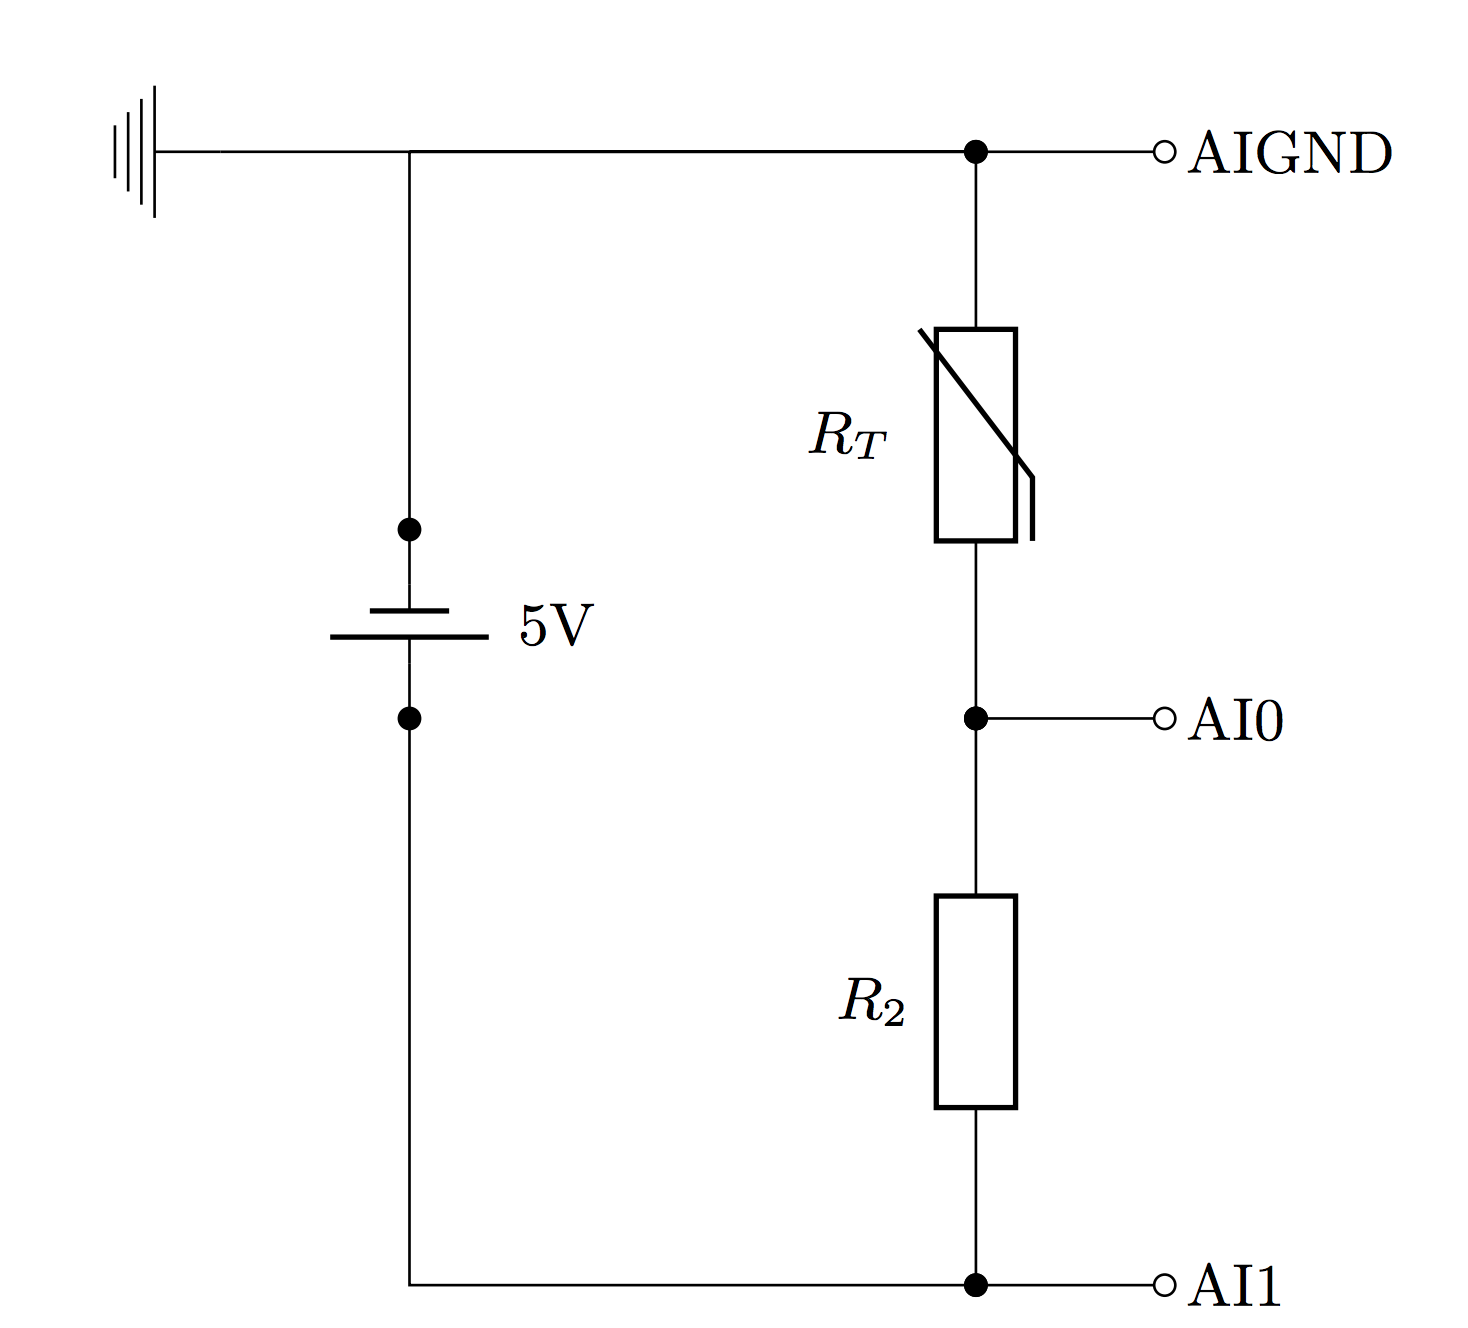
\includegraphics[scale=0.3]{fig_4.png}
    \caption{Elektrisk krets brukt for å måle $R_T$, og sende informasjon målinger gjennom en DA-omformer til datamaskinen. Ved å gi datamaskinen verdien til referansemotstand kan vi regne ut, og plotte temperaturen som en funksjon av tid. Formelen brukt for å regne ut temperaturen fra referansen er \eqref{calc_temp} \cite{oppgave}.}
    \label{fig4}
\end{figure}
Her er $R_T$ motstanden til en halvleder som er mer følsom mot temperaturforandring enn andre motstander. Ved at datamaskinen regner spenningsfallet over termistoren, og vet strømmen som går i kretsen, kan den regne ut resistansen til $R_T$ over tid, og dermed få data om temperaturen til termistoren. Først lot vi termistoren ikke oppleve temperaturforandring, for å se om resitansen var konstant, deretter varmet den opp ved kontakt med huden.
\subsection{Krets med frekvensavhengig respons}
Hittil har vi brukt likestrøm (DC), men nå ønsker vi å gjøre eksperimenter med vekselstrøm (AC). Vekselstrømmen skal komme fra en funksjonsgenerator innebygd i oscilloscopet (PicoScope 2000 Series). Med funksjonsgeneratoren kunne vi variere amplitude og frekvensen til signalet fra datamaskinen. Vi koblet F$45$ inn i kretsen for å måle spenningen, her må multimeteret være stilt inn på AC. Vi sammenlignet så verdien vi leste av på F$45$, med verdien vi valgte for spenningen med oscilloscopet. Vi gjorde dette for signaler med sinus, sagtann og firkantsignal. \\
Til slutt ønsker vi å se på forholdet mellom to spenningsfallet i en RC krets med vekselstrøm som fungerer som et lavpassfilet på grunn av tregheten i kondensatoren, kretsen er vist i figur \ref{fig5}. Vekselstrømmen skal komme fra en funksjonsgenerator innebygd i oscilloscopet (PicoScope 2000 Series) og fra DA-omformer (digital-to-analog-omformer). Vi kunne henholdsvis lese av signalet på datamaskinen ved hjelp av en oscilloscopet og AD-omformer (analog-to-digital-omformer) for å gjøre målinger på kretsen.
\begin{figure}[h!]
  \centering
  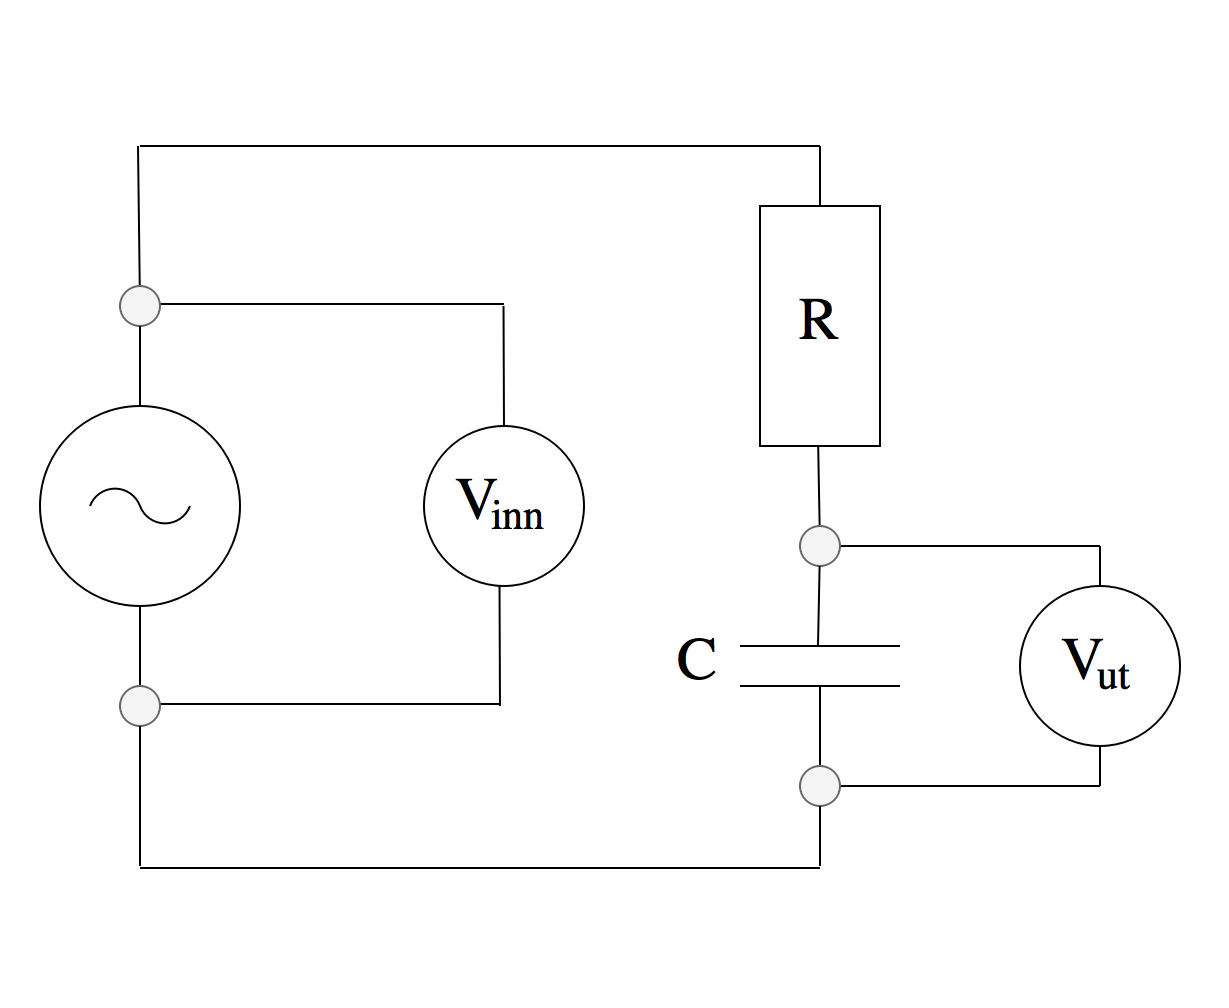
\includegraphics[scale=0.19]{fig_5.png}
  \caption{Krets brukt for å finne forholdet mellom $V_{inn}$ og $V_{ut}$ som blir forårsaket av tregheten i kondensatoren. De små sirklene ved batteriet representerer hvor vi koblet ledningene inn til først oscilloscopet, og senere til DA-omformeren for å generere signalet. De to små sirklene ved kondensatoren representerer hvor vi målte av dataen, først med oscilloscopet og senere med AD-omformeren for å sende data til datamaskinen.}
  \label{fig5}
\end{figure}
Som beskrevet i teoridelen (seksjon \ref{teori}) skaper kondensatoren en treghet i systemet hvis vi har en høy frekvens på spenningen i kretsen. For å gjøre målinger på denne effekten varierte vi frekvensen til et sinussignal fra spenningsgeneratoren logaritmisk fra $10$ til $10^6$ Hz, og gjorde noen ekstra målinger på området der vi merket forandring, som var for $500$, $5000$ og $50000$ Hz. Amplituden til signalet fra vekselstrømmen var på $\SI{706.5}{\milli \volt}$. For hver instilling noterte vi frekvens og amplitude til $V_{inn}$ og $V_{ut}$. Vi gjorde målingene først med oscilloscopet deretter med en AD-omformeren (anlog-to-digital-converter). Kapasitansen til kondensatoren var $\SI{100}{\nano\farad}$, og motstanden hadde resistans på $\SI{10}{\kilo\ohm}$.

\section{Resultater}
\subsection{Måling av multimetre}
Resultater fra måling av kretsen vist i tabell \ref{table1}. Dataen i denne tabellen kommer fra avlesninger av kretsen vist i figur \ref{fig1}, der vi bare hadde måleapparatene F$45$ og F$75$ i krets med hverandre og varierte hva apparatene målte. Fra denne dataen kan vi se hvordan måleapparatet selv påvirker kretsen de selv er med i. \\
\begin{table}[h!]
\caption{Data fra elektrisk krets kunn med måleapparater  F$45$ og F$75$. Kretsen som dataen er hentet fra er vist i figur \ref{fig1}. Ut fra enhetene til verdiene målt finner du hva de målte av hverandre. Verdiene inne i klammeparantese på de to øverste målingene vier sensitivteten til F$75$.}\centering
\label{table1}
\begin{tabular}{c c c}
\toprule
Fluke 75                 & Fluke 45                  & Rate F45 \\
\hline
$0.76 \pm  0.01$mA $[300$mA$]$       & $5.96 \pm 0.03 \Omega$ & S           \\
$0.00 \pm 0.02 $A $[10$A$]$       & $0.152 \pm 0.03 \Omega$  & S \\
$1.559 \pm 0.008$V       & $11.100 \pm 0.040 $M$\Omega$    & S        \\
$1.559 \pm 0.008$ V      & $11.10 \pm 0.03$M$\Omega$ & M        \\
$1.559 \pm 0.008$V       & $11.0 \pm 0.3 $M$\Omega$    & F        \\
$10.00 \pm 0.06$M$\Omega$  & $721.9 \pm 0.7 $mV       & S        \\
$10.00 \pm 0.06$M$\Omega$ & $0.7219 \pm 0.0004 $V   & M        \\
$10.02 \pm 0.06$M$\Omega$  & $0.720 \pm0.002$V         & F        \\
$0.000 \pm 0.001$V       & $0 \pm 1.5 \cdot 10^{-6}$ A     & S        \\
$0.000 \pm 0.001$V       & $0  \pm 3 \cdot 10^{-6}$ A      & M        \\
$0.000 \pm 0.001$V       & $0 \pm 3 \cdot 10^{-5}$ A       & F    \\
\end{tabular}
\end{table}
\subsection{Motstand, likestrøm og likespenningsmålinger
med multimeter}
Kretsen vist i figur \ref{fig2} ble brukt til å måle resistansen til to motstander. Målingene vi gjorde er vist i tabell \ref{table2}. \\
\begin{table}[h!]
\centering
\caption{Målinger gjort av F$45$ og F$75$, som måler resistansen til to kjente motstander. Kretsen for målingene er vist i figur \ref{fig2}.}
\label{table2}
\begin{tabular}{c c c c}
\toprule
Apparat & $\Omega$ oppgitt & $\Omega$ målt    & $\Delta \Omega$    \\
\hline
Fluke45 & $10\Omega$       & $10.141 \Omega$  & $\pm 0.009\Omega$ \\
Fluke75 & $10\Omega$       & $10.00\Omega$     & $\pm 0.15\Omega$    \\
Fluke45 & $1$ M $\Omega$   & $1.004$M$\Omega$ & $\pm 3.1$k$\Omega$ \\
Fluke75 & $1$ M $\Omega$   & $1.004$M$\Omega$ & $\pm 6$k$\Omega$   \\
\end{tabular}
\end{table}
I kretsen vist i figur \ref{fig3} målte vi spenningen over batteriet og over resistansen, og vi målte strømmen ved et ampermeter. Ved hjelp av Ohm's lov \eqref{ohm} kunne vi regne ut resistansen til motstanden. Dataen fra denne måkingen er vist i tabell \ref{table3}.
\begin{table}[h!]
\centering
\caption{Målingene gjort på kretsen vist i figur \ref{fig3}}
\label{table3}
\begin{tabular}{c c c c }
\toprule
    Strøm $I$ (mA) & Spenning $V$ (V) & Resistans $R = V/I$ (M$\Omega$) & Målested \\
\hline
 $ 0.0042 \pm 0.0015$  &   $4.22 \pm 0.03$ &                $  1.00 \pm 0.36 $ &      $V_{inn}$ \\
 $0.0046 \pm 0.0015$ &   $ 4.25 \pm 0.03$ &             $    0.92 \pm 0.31 $&     $ V_{ut} $\\
 $0.0060 \pm 0.0015$ &   $ 6.04 \pm 0.04$ &                 $ 1.01 \pm 0.26 $&     $ V_{inn}$ \\
 $0.0066 \pm 0.0015 $ &   $ 6.04 \pm 0.04$ &               $   0.92 \pm 0.21 $ &     $ V_{ut}$ \\
 $0.0081 \pm 0.0015$ &   $ 8.22 \pm 0.05$ &                 $ 1.01 \pm 0.19 $&     $ V_{inn}$ \\
$ 0.0089 \pm 0.0015$ &    $8.22 \pm 0.05$ &                  $0.92 \pm 0.16$ &      $V_{ut}$ \\
\end{tabular}
\end{table}
\subsection{Måle temperatur ved hjelp av resistanse}
Dataen fra kretsen vist i figur \ref{fig4} ble sendt til datamaskinen hvor vi kunne fremstlle temperaturen til termistoren som en funksjon av tid ved å regne ut resistansen med Ohm's lov \eqref{ohm}, og bruke \eqref{calc_temp} til å finne temperaturen. Grafen vist i figur \ref{fig6} viser hvordan temperaturen endrer seg over tid.
\begin{figure}[h!]
  \centering
  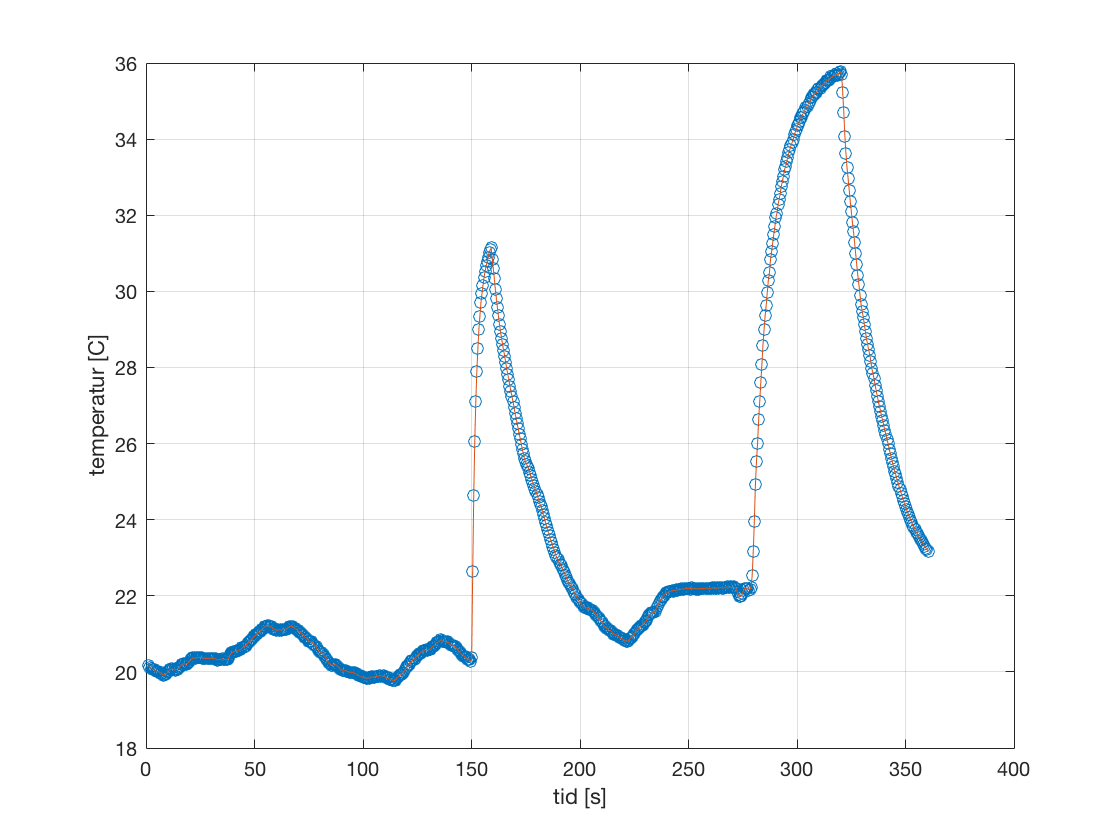
\includegraphics[scale=0.25]{fig_6.png}
  \caption{Temperaturen til termistoren som en funksjon av tid. Hver sirkel representerer en måling. Vi kan med dette lettere se hvor rask endringen er. Den oransje linja under er en linje trukekt mellom hver måling.}
  \label{fig6}
\end{figure}

\subsection{Vekselspenning med frekvensgenerator, oscilloscop og multimeter}
I den elektriske kretsen vist i figur \ref{fig5} varierte vi formen på signalet mellom sinus, sagtann og firkant-signal. Da vi leste av målingene gjort med oscilloscopet fant vi dataen vist i tabell \ref{table5}.
\begin{table}[h!]
\centering
\caption{Målingene gjort på kretsen vist i figur \ref{fig5}. Her er Amplituden den vi valgte på oscilloscopet, F$45$ er verdien vi leste av multimeteret, og RMS er RMS veriden til signalet, utregnet av oscilloscopet.}
\label{table5}
\begin{tabular}{c c c c}
\toprule
    Signalform & Amplitude $V$ (V) & F$45$ $V$ (mV)  & RMS(mV) \\ \hline
 Sinus   &    $1$  &                  $705.79 \pm 2.41$ &      $705.7 \pm 2.5 \cdot 10^{-4}$ \\
 Firkant &   $ 50$ &                  $49.627 \pm 0.20$ &      $50.6 \pm 0.0024$\\
 Sagtann &    $2$  &                  $1.1419 \pm 0.0214$ &    $1.149 \pm 3.5 \cdot 10^{-4}  $ \\
\end{tabular}
\end{table}
\subsection{Krets med frekvensavhengig respons}
Kretsen vist i figur \ref{fig5} ble først målt av oscilloscopet. Her målt vi $V_{ut}$, $V_{inn}$ og frekvensen $f$ til systemet. Målingene gjort er vist i figur \ref{fig7}. Her har vi funnet en lineærtilpassning til den $8$ høyeste frekvensene. Vi at stigningstallet var på $ -0.9363 \pm 0.063$. Vi fant konstantleddet til å være $1.9367 \pm  0.26$, men siden vi tok logaritmen av verdien går $V_{ut}/V_{inn}$ som $(35.61 \pm 9.26) \cdot 10^{-0.9363f \pm 0.063}$ . Fra denne tilpassnignskurven kan vi regne at $\log_{10} \abs{{V_{ut}/V_{inn}}} = 0$
skjer ved $\omega = 10^{2.0684 \pm 0.0111} = 117.06 \pm 1.29$
\begin{figure}[h!]
  \centering
  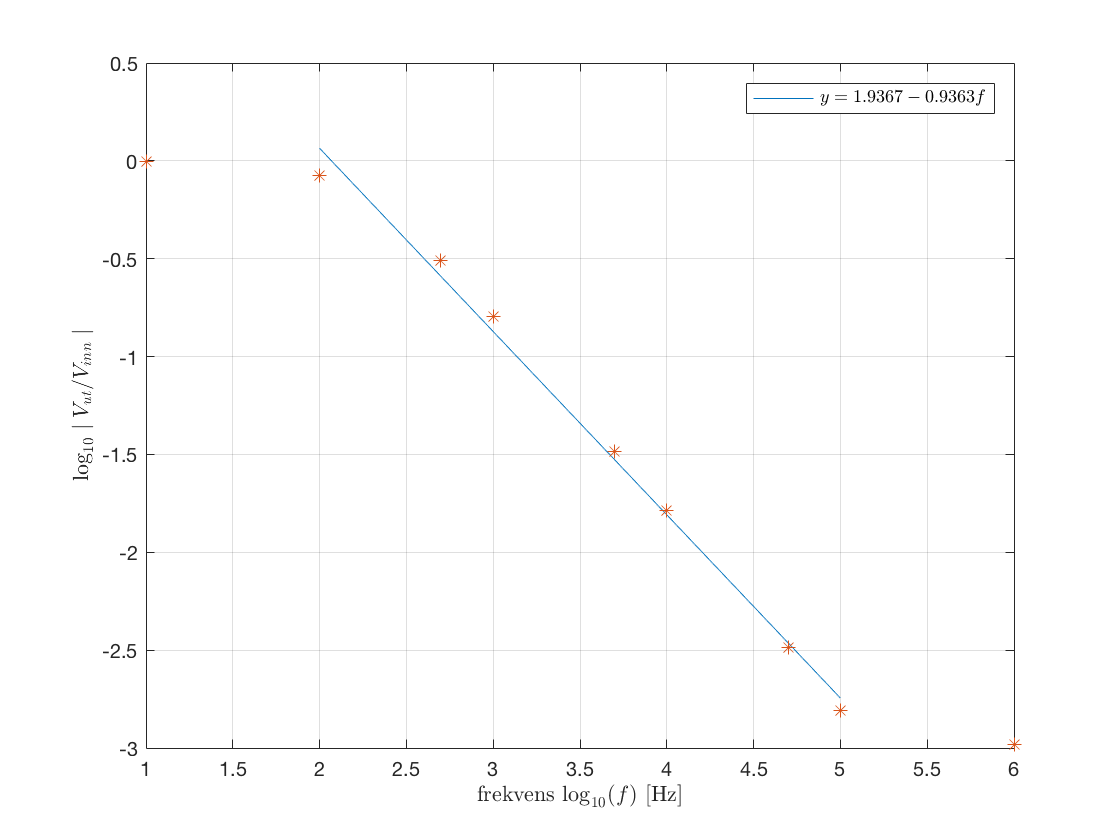
\includegraphics[scale=0.25]{fig_7.png}
  \caption{Forhold mellom spenning inn og ut av kretsen, plottet med logaritmisk akser. Dataen er hentet fra et oscilloscop. Her er usikkerhetene en faktor $10^{-3}$ iforholdet til avleste verdi, og det er derfor ikke mulige å se error-barene.}
  \label{fig7}
\end{figure}
Så gjorde vi de samme målingene med AD-omformeren. Målingene er vist i figur \ref{fig8}. Her målte vi $V_{ut}$, $V_{inn}$ og frekvensen $f$ til systemet. Her har vi funnet en lineærtilpassning til de $12$ siste punktene, det vil si etter knekken i grafen. Vi fant at stigningstallet var på $ -0.909 \pm 0.025$, og konstantleddet til å være $1.89 \pm  0.08$, men siden vi gjort det logaritimsk går $V_{ut}/V_{inn}$ som$ (77.75 \pm 6.12) \cdot 10^{-0.909f \pm 0.025}$.
Fra tilpassnignskurven kan vi regne at $\log_{10} \abs{{V_{ut}/V_{inn}}} = 0$ i $\omega = 10^{2.079 \pm 0.005} = 120.03 \pm 0.62$Hz.
Fra disse målingene fant vi at verdien for egenfrekvensen $\omega_0$ til systemet er på $118.54 \pm  0.68$Hz.
\begin{figure}[h!]
  \centering
  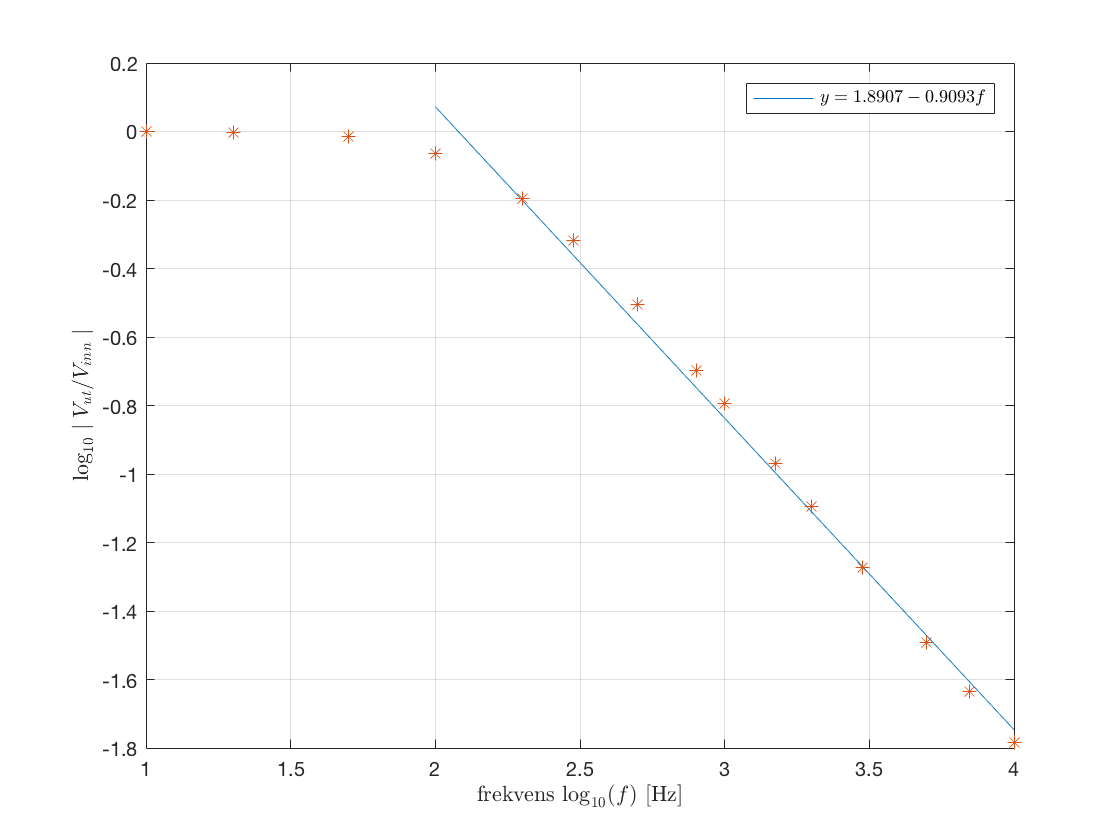
\includegraphics[scale=0.25]{fig_8.png}
  \caption{Forhold mellom spenning inn og ut av kretsen, plottet med logaritmisk akser. Dataen er hentet fra en AD-omformer. Her er usikkerhetene en faktor $10^{-3}$ iforholdet til avleste verdi, og det er derfor ikke mulige å se error-barene.}
  \label{fig8}
\end{figure}
\section{Diskusjon}
\subsection{Måling av multimetere}
Fra dataen vist i tabell \ref{table1} kan vi trekke flere sluttninger. Noe av det mest merkbare vi ser er at vi har målt null i de tre nederste radene for både strøm og spenning. Fra dette kan vi trekke slutningen at F$45$ og F$75$ ikke trenger å sende strøm gjennom kretsen for å måle spenning og strøm, men at de vil sende en strøm gjennom kretsen når de måler motstand. Vi ser også at voltmeteret i F$75$ har en indre resistanse på $11.10\pm0.07$M$\Omega$, og voltmeteret på F$45$ har en indre resistans på $10.00\pm0.06$M$\Omega$. For at det ikke skal gå noe strøm gjennom voltmeteret er det viktig at voltmeteret har en stor resistanse. Hvis resistansen F$75$ eller F$45$ måler spenningsfallet over en komponent som begynner å nærme seg en resistanse på $10$M$\Omega$ vil det være en merkbar effekt i verdien man leser av voltmeteret på grunn av påvirkningen voltmeteret har på kretsen. Når voltmeteret og motstanden nærmer seg lik motstand vil mye av strømmen gå gjennom voltmeteret, og spenningsfallet voltmeteret måler blir feil. Multimetere skal egentlig bare måle spenning, og her har vi sett hvorfor. For at et multimeter skal måle resistanse må den selv sende en strøm gjennom kretsen, som er langt fra ideelt. Og for at et multimeter skal måle strømmen gjennom kretsen vil multimeteret ha en resistanse, som er enten $5.958 \pm 0.03\Omega$ eller $0.15 \pm 0.03\Omega$ avhengig av sensitiviteten til multimeteret. Itillegg ser vi at F$75$ er litt bedre for å måle spenning over komponenter med høy motstand, men at F$45$ har en høyere nøyaktighet på målingene den gjør, og mulighet til å stille inn en verdi av samplings rateen.\\
\subsection{Motstand, likestrøm og likespenningsmålinger med multimeter}
Fra målingene vist i tabell \ref{table2} ser vi at F$45$ har en mye høyere nøyaktiget. For lave resistanser er den en faktor $100$ mer nøyaktig. Men når resistansen øker til $1$M$\Omega$ blir nøyaktigheten til begge multimeterene kraftig redusert. Grunnen til dette er at rekkevidde de skal måle over har økt, men det er like mange bits i måleapparatet, som nå må fordeles over et større intervall. For den store resistansen er F$45$ fortsatt mer nøyaktig, men forskjellen er bare på en faktor $0.5$.
\\
Når vi ser på målingene vist i tabell \ref{table3} ser vi en klar tendens. Målinger av motstanden med resistanse på $1$M$\Omega$ er mye nærmere den sanne verdien av resistansen når vi regner ut resistansen ved hjelp av spenningen målt på $V_{inn}$ istedenfor spenningen målt av  $V_{ut}$.
Grunnen til dette er at resistansen til motstanden er av samme størellsesorden som motstanden i voltmeteret som er koblet i paralellkobling for å måle spenningsfallet over motstanden. Målingene vist i tabell \ref{table1} vist oss at den indre motstanden til voltmeteret i F$45$ var på $11.10\pm0.07$M$\Omega$. For at et voltmeter skal gi en nøyaktig måling må den indre resistansen i voltmeteret være mye større enn motstanden til kompenten den måler spenningsfallet over. Siden dette ikke er sant når F$45$ måler spenningsfallet over en motstand på $1$M$\Omega$ får vi en systematisk feil i målingene våre. Årsaken er at en merkbar andel av strømmen går gjennom voltmeteret, og følgelig går mindre strøm gjennom resistansen, som gjør at vi måler en lavere resistanse på motstanden. Ideelt sett skal det ikke gå noe strøm gjennom voltmeteret.
Siden vi ikke hadde nok måleapparater målte vi ikke spenningsfallet over batteriet og spenningsfallet over resistansen samtidig. Derfor var, når vi målte spenningsfallet over hele kretsen med $V_{inn}$, tilnærmet lik all spenningsfallet i kretsen over motstanden på $1$M$\Omega$, siden motstanden fra amperemeteret er neglisjerbar. Vi fant i tabell \ref{table1} at motstanden til F$75$ som amperemter var på $0.15 \pm 0.03\Omega$, som er ingenting iforhold til 1M$\Omega$.
Vi ser fra tabellen \ref{table3} at vi får måler en resistanse nærmere den sanne verdiene av å regne ut motstanden ved å bare se på målinger fra $V_{inn}$. Hvis vi bare bruker verdier målt fra $V_{inn}$ får vi at $R = 1.006 \pm 0.159$M$\Omega$.
\subsection{Automatiserte målinger av termistor-motstand}
Av å måle verdier for termistormotstanden fra kretsen vist i figur \vref{fig3}, som er koblet med en AD-omformer som gir oss muligheten til å få målingene rett inn på datamaskinen klarte vi å finne temperaturen til termistoren over tid ved å bruke \eqref{calc_temp}. I kretsen brukte vi en referansemotstand som vi hadde målt til å være $1.006 \pm 0.159$M$\Omega$, som trengtes for utregningen av temperaturen.
\subsection{Vekselspenning med frekvensgenerator, oscilloscop og multimeter}
Fra målingene vist i tabell \ref{table5} ser vi at verdien vi måler fra multimeteret er lik RMS verdien til signalet. RMS-veriden represneterer arealet som kvadratet av signalet dekker på en hel periode. Uttrykket for RMS-verdien til en funksjon er \eqref{rms}, ved å vite formen på signalet og amplitude kan vi regne ut hva målingene fra multimeteret kommer til å være. For multimeteret vil nøyaktigheten av målingene være avhengig av frekvensen til signalet. For eksmpel vil F$45$ ha en nøyaktighet på $5\% + 500$ hvis signalet er mellom $50-100$kHz, mens hvis signalet er på mellom $25-50$Hz er nøyaktigheten på $1\%+100$, det er altså en faktor $5$ forskjell i nøyaktigheten. Det er derfor mer nøyaktig å lese av verdien direkte fra oscilloscopet. \\
Hvis vi hadde skrudd på en DC-komponent fra funksjonsgeneratoren i tillegg kunne vi ha funnet det på to forskjellige måter. Den første måten er at det hadde blitt en høyere avlesning på voltmeteret enn hva RMS-verdien til AC-signalet forutiser. Den andre måten er at vi kunne lese av verdien av \textit{hvile} amplituden, det vil si den amplituden AC-signalet svinger rundt, på dataskjermen koblet til funksjonsgeneratoren.
\subsection{Krets med frekvensavhengig respons}
Ut ifra dataen vist i figur \ref{fig7} og figur \ref{fig8} kunne vi regnet ut at $\log_{10} \abs{{V_{ut}/V_{inn}}} = 0$ fant sted når $118.54 \pm 0.68$Hz Hz. Dette betyr at for frekvenser som er mindre enn $118.54 \pm 0.68$ Hz vil vil ikke få en dempet respons grunnet treghet i kondensatoren. Men frekvenser større enn dette vil vi få en redusert amplitude, og den blir kraftigere redusert jo større frekvensen er. Fra figuren ser vi at det siste datapunktet passer dårlig inn med resten av datapunktene. Dette gir oss grunn til å tro at det var en systematisk feil til stedet under målingen av dette datapunktet, og at dette ville forårsaket en lavere verdi for $\log_{10} \abs{{V_{ut}/V_{inn}}}$. Vi tok derfor valget å ikke ta med dette datapunktet i lineærregersjonen. Dette kan tyde på at det burde gjøres flere eksperimenter i dette frekvensområdet.\\
I teori-delen i seksjon \ref{teori} fant vi at konstantleddet vi finner for høye frekvenser skal være tilnærmet lik $\omega_0$. I kretsen vår brukte vi en resistanse på $10$k$\Omega$ og en kapasitans på $100$nF. Siden $\omega = 1/RC$, skal $\omega_0$, ifølge teorien, være $10^3$Hz. Vi har målt $\omega_0$ til å være $118.54\pm0.68$Hz. Grunnet at de eksperimentelle målingene avviker med en faktor på $10$, må da ha vært noe som forårsaket en systematisk feil under målingene. Den systematiske feilen gjorde at datapunktene er feil, og ikke passer inn med det teorien forutsier, som gjør at vi finner en gal verdi for $\omega_0$. Derfor er verdien funnet i disse målingene feil, og man skal ikke trekke noen slutninger fra disse målingene. \\
Det at vi målte så forskjellig $\omega_0$ ved de to forskjellige måltemetodene tyder også på at det var systematiske feil til stedet. Siden vi måler på samme krets, og med samme strøm, burde resultatet være likt. Den eneste forandringen er er at vi i det ene tilfellet henter dataen ved hjelp av picoscopet, og i det andre tilfellet ved hjelp av en AD-omformer.
\section{Konklusjon}
Ved å sette opp de elektriske kretsene vist i denne rapporten, har vi lært hvordan komponentene og måleapparatene virker i samspill med hverandre. Dette har vi gjort ved å gjøre målinger på spenning, strøm og motstand i kretsen, og få informasjon om egenskapene til kretsen ved hjelp av disse målingene. \\
Fra målingene har vi sett at man må vite hvordan måleapparartene påvirker kretsen. Vi fant at den indre resistansen til voltmeteret i F$45$ var på $10.00 \pm 0.06$M$\Omega$, og indre resistansen til F$75$ var på $11.10 \pm 0.07$M$\Omega$. Måleapparater er selv en del av kretsen, og vil følgelig påvirke den, og dette vil påvirke verdiene man måler. Fra å vite den indre resistansen til voltmeteret kan vi finne ut til hvilken grad voltmeteret påvirker kretsen. Vi fant at for at et multimeter skal kunne måle resistanse eller strøm kommer den til å selv produsere en strøm i kretsen. \\For å måle resistansen vist i figur \ref{fig2} var det fordelaktig å måle resistansen over hele kretsen istedenfor over motstanden. Grunnen til dette var at resistansen til motstanden var av samme størrelsesorden som den indre resistansen til voltmeteret i paralell. Ved å måle resistansen over hele kretsen istedenfor i paralell fant vi at verdien til resistansen var $1.006\pm0.159$M$\Omega$. \\
Ved å måle resistansen til en temperatursensitiv motstand, termistor, og vite forholdet mellom resistansen til motstanden og temperaturen \eqref{calc_temp} klarte vi å finne temperaturen til termistoren. \\
Vi gjorde målinger på en krets med en spenningsgenator hvor vi kunne variere formen, amplituden og frekvensen til signalet fant vi at multimeteret målte at spenningen var lik RMS-verdien til formen av signalet. RMS-verdien er definert av \eqref{rms} og sier oss hva roten av arealet under grafen til spenningsformen kvadret over en full periode er, og det er denne verdien multimeteret måler. \\
Den elektriske kretsen vist i figur \ref{fig8} og figur \ref{fig7} fungerer som et lavpassfilter. Hvis man har en påtrykkt spenning med frekvens vil kondensatoren lades opp med ladninger, men hvis frekvensen er høy nok vil ikke kondensatoren rekke å bli ladet opp før spenningen har endret seg. Derfor vil signalene med høy frekvens få en sterkt dempet amplitude. Hvis vi plotter påtrykkt frevens mot potensialforskjell logaritmisk kan vi finne den karakteristiske frekvensen til systemet $\omega_0$ ved hjelp av lineær regresjon. Eksperimentet ga oss at denne verdien var på $118.54 \pm 0.68$Hz. Under oppsettningen av vårt eksperimentet ble noe gjort galt, og vi fant feil verdi for den karakteristiske frekvensen til systemet på grunn av systematiske feil i eksperimentet. Det burde bli gjort mer eksperimenter for å finne $\omega_0$ eksperimentelt.
\begin{thebibliography}{9}
\bibitem{squires}
Squires, G.L. \emph{Practical Physics}, Cambridge University Press, 2001.
\bibitem{skaar}
Skaar, J. \emph{Elektromagnetisme}, 2017
\bibitem{oppgave}
Dysthe, D.K\,\, Røyne, A.\,\, Ulven, O.I \emph{Strøm og spenning}, 2018

\bibitem{rms_wiki}
Wikipedia \emph{Root mean square}, 07.02.2018

\end{thebibliography}
\end{document}
%
% ****** End of file apssamp.tex ******
